\chapter{Implementation and Realization}
\minitoc % Generates a mini table of contents for this chapter

\section*{Introduction}
This chapter presents the implementation of the ERP backend system carried out during the internship at Anter Lab. 
The work followed the Scrum methodology, divided into four weekly sprints due to the one-month duration of the internship. 
Each sprint focused on specific objectives: environment setup, core administrative APIs, configuration management, and reporting. 
In addition, we illustrate the design with UML diagrams (use case, class, sequence) and provide scenario tables for selected modules.

% Include each sprint file
\section{Sprint 0: Environment \& Project Setup}

\subsection{Objectives}
Sprint 0 was dedicated to laying the groundwork for the ERP backend system. 
The main goal was to establish a stable and collaborative development environment, ensuring all team members shared the same technical foundation. 
This sprint also introduced initial API scaffolding, which served as the backbone for future sprints.

\subsection{Tasks Completed}

\paragraph{1. Project Initialization and Source Control}
\begin{itemize}
    \item Cloned the ERP backend project from the private GitLab repository.
    \item Verified and configured the development branch, ensuring proper synchronization with GitLab’s version control system.
    \item Established branching strategy (\texttt{main}, \texttt{develop}, feature branches) to support parallel work.
\end{itemize}

\paragraph{2. Environment and Database Setup}
\begin{itemize}
    \item Installed necessary dependencies for Laravel and PHP (via Composer).
    \item Configured the \texttt{.env} file for database connection and environment-specific settings.
    \item Created and migrated the MySQL database schema.
    \item Seeded initial data (roles, admin user) for authentication testing.
\end{itemize}

\paragraph{3. Communication and Project Management Tools}
\begin{itemize}
    \item Joined the ClickUp workspace, where the product backlog and sprint tasks were organized.
    \item Integrated into the Discord server for team communication, enabling daily stand-ups and instant collaboration.
    \item Defined the workflow of tracking tasks (To Do, In Progress, Done).
\end{itemize}

\paragraph{4. API Foundations}
\begin{itemize}
    \item Migrated the legacy \texttt{DashboardController} into REST API endpoints to align with modern backend architecture.
    \item Developed the first set of APIs:
    \begin{itemize}
        \item \texttt{POST /register} – User registration endpoint.
        \item \texttt{POST /login} – JWT-based authentication endpoint.
        \item \texttt{GET /user-info} – Fetch authenticated user profile and roles.
    \end{itemize}
    \item Documented these endpoints and tested them in Postman.
\end{itemize}

\subsection{Outputs}
By the end of Sprint 0, the following deliverables were achieved:
\begin{itemize}
    \item A fully functional Laravel project running locally with database integration.
    \item Secure JWT authentication flow in place (Register, Login, User Info).
    \item A collaborative workflow using GitLab (source control), ClickUp (task management), and Discord (communication).
    \item A clear project roadmap established through backlog prioritization.
\end{itemize}

% --------------------------------------------------------
% USE CASE DIAGRAM
% --------------------------------------------------------
\subsection{Authentication Use Case Diagram}
\begin{figure}[H]
    \centering
    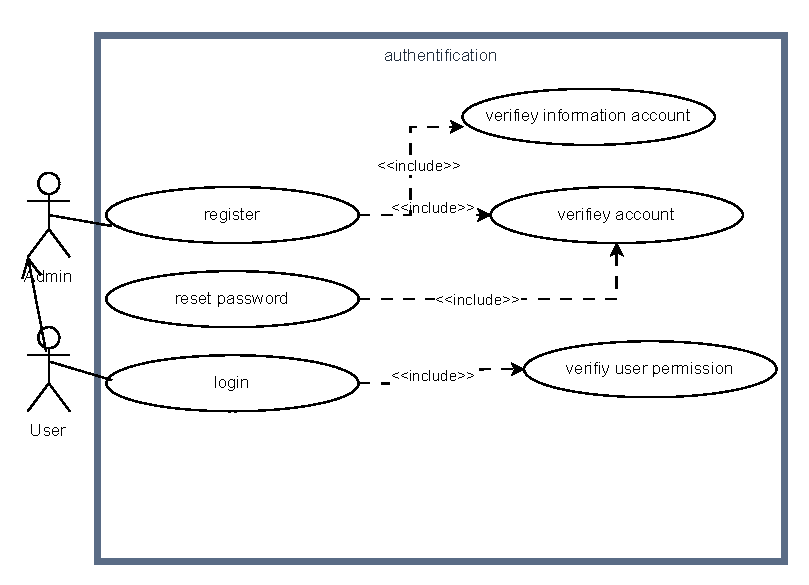
\includegraphics[width=0.85\textwidth]{chapters/chapter 3/figures/AuthUseCase.drawio_cropped.pdf}
    \caption{Specific Use Case Diagram for Authentication APIs}
    \label{fig:sprint0_usecase}
\end{figure}

% --------------------------------------------------------
% USE CASE SCENARIO TABLE
% --------------------------------------------------------
\subsection{Use Case Scenario: User Login}
\begin{longtable}{|p{3cm}|p{11cm}|}
\hline
\textbf{Use Case} & User Login with JWT \\
\hline
\textbf{Actor} & Registered User \\
\hline
\textbf{Preconditions} & 
\begin{minipage}[t]{10cm}
\begin{itemize}
    \item User already registered in the system.
    \item Database contains valid user credentials.
\end{itemize}
\end{minipage} \\
\hline
\textbf{Main Flow} &
\begin{minipage}[t]{10cm}
\begin{enumerate}
    \item User enters email and password.
    \item System verifies credentials against database.
    \item If valid, system generates JWT token.
    \item System returns token and user details to client.
\end{enumerate}
\end{minipage} \\
\hline
\textbf{Alternative Flows} &
\begin{minipage}[t]{10cm}
\begin{itemize}
    \item Invalid credentials → System returns error message.
    \item Missing data → System prompts user to re-enter credentials.
\end{itemize}
\end{minipage} \\
\hline
\textbf{Postconditions} & 
\begin{minipage}[t]{10cm}
User is authenticated, token stored for accessing protected APIs.
\end{minipage} \\
\hline
\caption{Use Case Scenario: User Login}
\label{tab:usecase_login}
\end{longtable}
% --------------------------------------------------------
% SEQUENCE DIAGRAM
% --------------------------------------------------------
\subsection{Sequence Diagram: User Login Flow}
\begin{figure}[H]
    \centering
    \includegraphics[width=0.9\textwidth]{chapters/chapter 3/figures/sequence_DG_Auth.png}
    \caption{Sequence Diagram for Login API}
    \label{fig:sprint0_sequence}
\end{figure}

% --------------------------------------------------------
% CLASS DIAGRAM
% --------------------------------------------------------
\subsection{Class Diagram: Authentication Module}
\begin{figure}[H]
    \centering
    \includegraphics[width=0.85\textwidth]{chapters/chapter 3/figures/class_diagram.png}
    \caption{Class Diagram for Authentication Entities}
    \label{fig:sprint0_class}
\end{figure}

\subsection{API Testing with Postman}
To validate the core authentication APIs, Postman was used for sending HTTP requests and verifying responses. The following figures illustrate the results of the \texttt{Register}, \texttt{Login}, and \texttt{/user} (getUserInfo) endpoints.

\begin{figure}[H]
    \centering
    \includegraphics[width=0.8\textwidth]{chapters/chapter 3/figures/register.png}
    \caption{Postman Test -- Register API (Successful User Registration)}
    \label{fig:postman_register}
\end{figure}

\begin{figure}[H]
    \centering
    \includegraphics[width=0.8\textwidth]{chapters/chapter 3/figures/login.png}
    \caption{Postman Test -- Login API (Authentication with JWT)}
    \label{fig:postman_login}
\end{figure}

\begin{figure}[H]
    \centering
    \includegraphics[width=0.8\textwidth]{chapters/chapter 3/figures/user.png}
    \caption{Postman Test -- /user API (Fetching Authenticated User Information)}
    \label{fig:postman_user}
\end{figure}

\section{Sprint 0: Dashboard API Endpoints (HRM Example)}

\subsection{Objectives}
The objective of this part of Sprint 0 was to migrate the legacy Dashboard features into REST API endpoints and make them available for the ERP backend.  
The dashboard contains several modules such as HRM, POS, CRM, Accounting, and general system monitoring. In this section, we focus on the HRM (Human Resources Management) dashboard as a representative example.

\subsection{Main Endpoints (Dashboard APIs)}
The following endpoints were implemented and tested in Sprint 0:
\begin{itemize}
    \item \texttt{GET /dashboard-index} – Main dashboard overview.
    \item \texttt{GET /crm-dashboard} – CRM module summary.
    \item \texttt{GET /hrm-dashboard} – HRM module summary.
    \item \texttt{GET /pos-dashboard} – POS (Point of Sale) overview.
    \item \texttt{GET /account-dashboard-index} – Accounting/Finance summary.
    \item \texttt{GET /order-chart} – Charts for orders and transactions.
    \item \texttt{GET /get-projects} – Projects overview.
\end{itemize}

\subsection{Use Case: HRM Dashboard}
The HRM dashboard aggregates employee management, payroll, attendance, and recruitment data for managers and admins. Figure~\ref{fig:hrm_use_case} shows the use case diagram.

\begin{figure}[H]
    \centering
    \includegraphics[width=0.9\textwidth]{chapters/chapter 3/figures/diagramGeneralUseCase (1) (1).drawio (1).pdf}
    \caption{HRM Dashboard Use Case Diagram}
    \label{fig:hrm_use_case}
\end{figure}

\subsection{Detailed Scenario: Manage Employees (HRM Dashboard)}
\begin{longtable}{|p{3cm}|p{11cm}|}
\hline
\textbf{Use Case} & Access HRM Dashboard \\
\hline
\textbf{Actor} & Admin \\
\hline
\textbf{Preconditions} &
\begin{minipage}[t]{10cm}
\begin{itemize}
    \item Admin is authenticated and has a valid JWT token.
    \item The HRM module is active.
\end{itemize}
\end{minipage} \\
\hline
\textbf{Main Flow} &
\begin{minipage}[t]{10cm}
\begin{enumerate}
    \item Admin navigates to the HRM section of the application.
    \item The system automatically sends a request: \texttt{GET /hrm-dashboard} (with JWT token in header).
    \item The system verifies the token and retrieves HRM dashboard data.
    \item The system returns a successful response containing dashboard data.
    \item The application displays the HRM dashboard to the administrator.
\end{enumerate}
\end{minipage} \\
\hline
\textbf{Alternative Flows} &
\begin{minipage}[t]{10cm}
\begin{itemize}
    \item \textbf{A1: Invalid / Missing JWT token:} System returns \texttt{401 Unauthorized}. Redirect to login.
    \item \textbf{A2: Empty Dashboard Data:} System returns \texttt{200 OK} with empty object → app displays empty dashboard.
\end{itemize}
\end{minipage} \\
\hline
\textbf{Postconditions} & 
\begin{minipage}[t]{10cm}
The HRM dashboard is successfully loaded and displayed to the authenticated Admin.
\end{minipage} \\
\hline
\caption{Use Case Scenario: Accessing the HRM Dashboard (Sprint 0)}
\label{tab:usecase_hrm_dashboard}
\end{longtable}


\subsection{Sequence Diagram: Dashboard Controller}
\begin{figure}[H]
    \centering
    \includegraphics[width=0.9\textwidth]{chapters/chapter 3/hrmFigures/sequence_DG_hrm.png}
    \caption{Sequence Diagram for Login API}
    \label{fig:sprint0_sequence}
\end{figure}

\subsection{Class Diagram: HRM Dashboard }
\begin{figure}[H]
    \centering
    \includegraphics[width=0.85\textwidth]{chapters/chapter 3/hrmFigures/class_diagram_hrm.png}
    \caption{Class Diagram for Authentication Entities}
    \label{fig:sprint0_class}
\end{figure}

\subsection{API Testing with Postman}
To validate the core dashboard APIs implemented in Sprint 0, Postman was used for sending HTTP requests and verifying responses. The following figures illustrate the successful responses from the key endpoints, all of which require a valid JWT Bearer Token for authorization. A known issue with the HRM module is also documented.

\begin{figure}[H]
    \centering
    \includegraphics[width=0.8\textwidth]{chapters/chapter 3/hrmFigures/gt-dashboard-index.png}
    \caption{Postman Test -- GET /api/get-dashboard-index (Retrieving Main Dashboard Metrics)}
    \label{fig:postman_main_dashboard}
\end{figure}

\begin{figure}[H]
    \centering
    \includegraphics[width=0.8\textwidth]{chapters/chapter 3/hrmFigures/account-dashboard.png}
    \caption{Postman Test -- GET /api/get-account-dashboard-index-api (Retrieving Financial Dashboard Data)}
    \label{fig:postman_account_dashboard}
\end{figure}

\begin{figure}[H]
    \centering
    \includegraphics[width=0.8\textwidth]{chapters/chapter 3/hrmFigures/oder_chart.png}
    \caption{Postman Test -- GET /api/order-chart (Retrieving Sales Chart Data)}
    \label{fig:postman_order_chart}
\end{figure}

\begin{figure}[H]
    \centering
    \includegraphics[width=0.8\textwidth]{chapters/chapter 3/hrmFigures/crm-dashboard.png}
    \caption{Postman Test -- GET /api/crm-dashboard (Retrieving CRM Metrics)}
    \label{fig:postman_crm_dashboard}
\end{figure}

\begin{figure}[H]
    \centering
    \includegraphics[width=0.8\textwidth]{chapters/chapter 3/hrmFigures/pos_dashboard.png}
    \caption{Postman Test -- GET /api/pos-dashboard (Retrieving Point-of-Sale Data)}
    \label{fig:postman_pos_dashboard}
\end{figure}

\begin{figure}[H]
    \centering
    \includegraphics[width=0.8\textwidth]{chapters/chapter 3/hrmFigures/get-projects.png}
    \caption{Postman Test -- GET /api/get-projects (Retrieving Project List)}
    \label{fig:postman_get_projects}
\end{figure}

\begin{figure}[H]
    \centering
    \includegraphics[width=0.8\textwidth]{chapters/chapter 3/hrmFigures/hrm_employee_not_found.png}
    \caption{Postman Test -- GET /api/hrm-dashboard (Endpoint Routed but Not Implemented - 404 Status)}
    \label{fig:postman_hrm_404}
\end{figure}

%\section{Sprint 1: Core Administrative APIs}

\subsection{Objectives}
Sprint 1 focused on building the foundational administrative APIs that define the company’s structure and workforce.  
The main goal was to implement full CRUD operations for Employees, Branches, Departments, and Designations, ensuring all entities could be created, updated, deleted, and retrieved securely.  
Bulk operations such as Import/Export for Employees were also introduced.

\subsection{Tasks Completed}
\begin{itemize}
    \item Implemented CRUD APIs for the following entities:
    \begin{itemize}
        \item Employees (with Import \& Export functionality).
        \item Branches.
        \item Departments.
        \item Designations.
    \end{itemize}
    \item Secured all endpoints with JWT authentication middleware.
    \item Documented endpoints and tested responses in Postman.
    \item Updated database schema to support relations (Employees linked to Departments, Branches, and Designations).
\end{itemize}

\subsection{Outputs}
By the end of Sprint 1, the following deliverables were achieved:
\begin{itemize}
    \item Functional APIs for organizational entities.
    \item Secure JWT-protected CRUD endpoints.
    \item Initial dataset for Employees, Branches, Departments, and Designations.
    \item Verified API responses through Postman.
\end{itemize}

% --------------------------------------------------------
% USE CASE DIAGRAM
% --------------------------------------------------------
\subsection{Administrative Use Case Diagram}
\begin{figure}[H]
    \centering
    \includegraphics[width=0.85\textwidth]{chapters/chapter 3/sprint1_figures/use_case_Employee-managment.png}
    \caption{Use Case Diagram for Administrative APIs (Employees, Branches, Departments, Designations)}
    \label{fig:sprint1_usecase}
\end{figure}

% --------------------------------------------------------
% USE CASE SCENARIO TABLE
% --------------------------------------------------------
\subsection{Use Case Scenario: Create Employee}
\begin{longtable}{|p{3cm}|p{11cm}|}
\hline
\textbf{Use Case} & Create Employee Record \\
\hline
\textbf{Actor} & Admin \\
\hline
\textbf{Preconditions} & 
\begin{itemize}
    \item Admin is authenticated with a valid JWT token.
    \item The system has at least one Branch, Department, and Designation defined.
\end{itemize} \\
\hline
\textbf{Main Flow} &
\begin{enumerate}
    \item Admin selects ``Add Employee'' option in the application.
    \item System sends a \texttt{POST /employees} request with employee details (name, email, salary, branch\_id, department\_id, designation\_id).
    \item API validates request payload.
    \item API stores the new employee in the database.
    \item System returns a \texttt{201 Created} response with employee details.
\end{enumerate} \\
\hline
\textbf{Alternative Flows} &
\begin{itemize}
    \item \textbf{A1: Missing/Invalid Token:} System returns \texttt{401 Unauthorized}.
    \item \textbf{A2: Invalid Data:} System returns \texttt{422 Unprocessable Entity} with validation errors.
    \item \textbf{A3: Foreign Key Missing:} If Branch/Department/Designation ID does not exist, system returns \texttt{404 Not Found}.
\end{itemize} \\
\hline
\textbf{Postconditions} & 
\begin{itemize}
    \item A new employee record is created and stored in the database.
    \item Employee is now linked to Branch, Department, and Designation entities.
\end{itemize} \\
\hline
\caption{Use Case Scenario: Create Employee (Sprint 1)}
\label{tab:usecase_create_employee}
\end{longtable}

% --------------------------------------------------------
% SEQUENCE DIAGRAM
% --------------------------------------------------------
\subsection{Sequence Diagram: Create Employee}
\begin{figure}[H]
    \centering
    \includegraphics[width=0.9\textwidth]{}
    \caption{Sequence Diagram for Create Employee API}
    \label{fig:sprint1_sequence}
\end{figure}

% --------------------------------------------------------
% CLASS DIAGRAM
% --------------------------------------------------------
\subsection{Class Diagram: Administrative Entities}
\begin{figure}[H]
    \centering
    \includegraphics[width=0.85\textwidth]{chapters/chapter 3/sprint1_figures/class_diagram_s1.png}
    \caption{Class Diagram for Employees, Branches, Departments, and Designations}
    \label{fig:sprint1_class}
\end{figure}

% --------------------------------------------------------
% API TESTING WITH POSTMAN
% --------------------------------------------------------
\subsection{API Testing with Postman}
The CRUD endpoints were tested using Postman to ensure correct functionality. Below are placeholders for screenshots:

\begin{figure}[H]
    \centering
    \includegraphics[width=0.8\textwidth]{chapters/chapter 3/sprint1Figures/postman_create_employee.png}
    \caption{Postman Test -- Create Employee API}
    \label{fig:postman_create_employee}
\end{figure}

\begin{figure}[H]
    \centering
    \includegraphics[width=0.8\textwidth]{chapters/chapter 3/sprint1Figures/postman_get_employees.png}
    \caption{Postman Test -- Get All Employees API}
    \label{fig:postman_get_employees}
\end{figure}

\begin{figure}[H]
    \centering
    \includegraphics[width=0.8\textwidth]{chapters/chapter 3/sprint1Figures/postman_update_employee.png}
    \caption{Postman Test -- Update Employee API}
    \label{fig:postman_update_employee}
\end{figure}

\begin{figure}[H]
    \centering
    \includegraphics[width=0.8\textwidth]{chapters/chapter 3/sprint1Figures/postman_delete_employee.png}
    \caption{Postman Test -- Delete Employee API}
    \label{fig:postman_delete_employee}
\end{figure}

%\input{chapters/chapter3/sprint2}
%\input{chapters/chapter3/sprint3}

\section*{Conclusion}
The implementation phase transformed the specifications into a functional ERP backend system. 
Through iterative sprints, we ensured continuous progress and adaptability. 
This chapter showcased the environment setup, API development, configuration options, and reporting features, supported by UML diagrams and scenarios. 
The next chapter will evaluate the testing and validation of the developed system.
